\documentclass[a4paper,12pt]{report}
\usepackage{amsmath, amsfonts, amssymb}
\usepackage{graphicx}
\usepackage{float}

\begin{document}

\begin{figure}
\begin{center}

\includegraphics[scale=0.6]{xidianU}
\end{center}
\end{figure}
\begin{figure}[htb]
\begin{center}
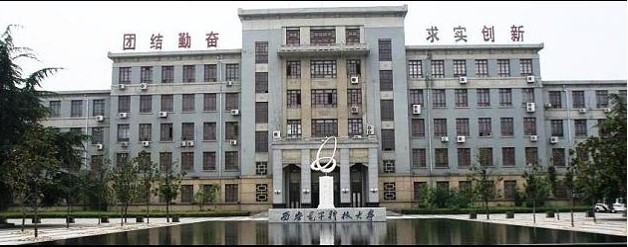
\includegraphics[scale=0.4]{xidianU1}
\end{center}
\end{figure}
$$$$
$$$$
$$$$
$$$$
\begin{center}
\textbf{Report on Operational Statistics for SAR I classes}
\textbf{Analysis of the rural image taken in Grubem}
\end{center}
$$$$
$$$$
$$$$

\begin{flushright}
\textbf{Name: Pedro Bartolomeu Nguendji}

\textbf{Number: 19036110002}
\end{flushright}

$$$$


\begin{center}
\textbf{2019, Xi’an}
\end{center}


\begin{flushleft}
\textbf{Introduction}
\end{flushleft}

SAR is short for Synthetic Aperture Radar. This is a special radar technique that allows users to take high-resolution radar images over long distances, e.g. eg from space. With radar microwaves are used to measure distances (amplitudes).
Unlike a sending radar altimeter for the nadir, the SAR system sends radar pulses to the side. Through the principle of lateral observation, the radar returns signals from different objects on Earth to the sensor at different times. This allows discriminating the objects. Side-view radar pulses form image lines (ie amplitude dimension). Another image dimension (i.e. azimuth dimension) is formed by the movement and direction of the sensor, which continuously sends and receives radar pulses.
 
\begin{flushleft}
\textbf{Image analysis in studies}
\end{flushleft}
SAR images are useful for studying the characteristics of ice and snow, as well as their changes over time. In addition, ice flow can be measured from repeated SAR images using image correlation (often referred to as "dot tracking" for SAR images).
Radar and SAR record the time of a return pulse and its intensity, as well as the microwave phase. These phase signals produce an interferogram between two SAR data acquisitions. Radar interferometry (InSAR) is used to measure ground elevations, while differential InSAR (DInSAR) is used to measure ground displacements such as glacier flow.$$$$

Figure 1 is a radar interferogram of the Gruben area. Color cycles are similar to contour lines and show the terrain topography as seen by the InSAR sensor. In the three areas indicated by the blue arrows, the color cycles are strongly distorted between the two SAR images that form the interferogram (see the three glaciers in a plane photograph of the Gruben area in the Swiss Alps.

	\begin{figure}[H]
	\begin{center}
	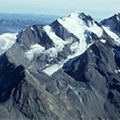
\includegraphics[scale=1]{fig1}
	\caption{Photograph of the Grubem area in the Swiss Alps, taken from an airplane}
	\end{center}
	\end{figure}
	
If the ice were not moving, the color cycles (ie fringes) would be parallel to the contour lines. In fact, the color cycles in the first interferogram (figure1) over the terrain around the glaciers look very similar to the color cycles that were simulated in an elevation model (second interferogram in figure 2).

	\begin{figure}[H]
	\begin{center}
	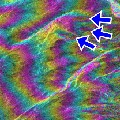
\includegraphics[scale=1]{fig2}
	\caption{Interferogram Over Gruben Area}
	\end{center}
	\end{figure}
	
On the other hand, when the terrain is not moving, contour lines can be calculated from an interferogram and a derived digital elevation model. In the three glaciers, however, color cycles are not only caused by topography, but also by daily ice movement between two acquisition dates.

If we know the topography of the area, we can simulate the topographic fringes (figure 2) and, as such, separate the topographic and ice dynamics contribution to color cycles by simply subtracting the simulated topographic fringes (second image) from the original interferogram that contains both topographic and motion fringes (figure 1)\ref{fig1}. Therefore, we can measure the movement of the ice with very high accuracy (figure 3).
\begin{figure}[H]
	\begin{center}
	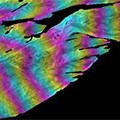
\includegraphics[scale=1]{fig3}
	\caption{Topography-only interferogram simulated from a digital elevation model}
	\end{center}
	\end{figure}
In summary, on stable ground, SAR interferometry can be used to measure terrain elevations, e.g. eg in a glacier. On unsteady terrain (eg floating glaciers) SAR interferometry can be used to measure ice movement with high accuracy. If more than one pair of SAR images are available, the two techniques can be combined to simultaneously measure glacier elevation and movement.
\begin{figure}[H]
	\begin{center}
	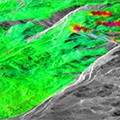
\includegraphics[scale=1]{fig4}
	\caption{Calculated displacement as the difference between the original interferogram and the simulated topographic interferogram}
	\end{center}
	\end{figure}
	
	\begin{flushleft}
\textbf{Conclusion}
\end{flushleft}

We can conclude that RADAR has some features that make it stand out over optical detectors, which stand out:

a)the interaction of radiation with clouds or radiation is reduced or even nullified due to the high wavelength;

b)while reflectance in optical detector images is related to the molecular properties of objects, RADAR images depend on macroscopic surface characteristics such as roughness, dielectric properties (related to moisture content), geometric characteristics of urban areas, structural characteristics of vegetation, the orientation of structures relative to beam direction of view, etc .;

c)images have a good spatial resolution, are obtained under any weather conditions, day or night and regardless of lighting conditions; These features make RADAR images very useful for surface monitoring in high cloud areas.


\end{document}